%\subsection{Einleitung}
Wie im Kapitel Daemon \ref{sec:daemon} schon angedeutet, ist der Grund für das Verwenden einer Datenbank einerseits den Beschränkungen der Twitter-API geschuldet, andererseits erlaubt uns die Verwendung einer eigenen Datenbank, Twitter-Daten zu erweitern (z.\,B. durch Sentimentwerte).
%Eine relationale Datenbank erlaubt es uns, alle für uns relevanten Daten zu speichern und erst später beliebige Anfragen auf diesen Daten auszuführen.
%Da sich erst im Laufe des Projektseminars herausstellte, welche Werte eines Datensatzes für uns interessant sind, kommt uns dieser Arbeitsansatz sehr entgegen. 
Wie in Kapitel \ref{sec:Tech} erwähnt, wird in unserem Projekt die Datenbank MySQL verwendet.
%TODO Ref

%\subsection{MySQL}
%Die Wahl ist recht schnell auf eine relationale Datenbank, genauer gesagt MySQL, gefallen.
%Das liegt hauptsächlich daran, dass ein Großteil der Projektseminar-Teilnehmer am meisten Erfahrungen mit %SQL und MySQL hatten.
%Wir haben zwar schon von der NoSQL-Datenbank gehört, da diese sich aber deutlich von relationalen Datenbanken unterscheidet, haben wir davon abgesehen, eine solche einzusetzen.
%Der mögliche Einarbeitungsaufwand in ein vollkommen neues System (wie zum Beispiel eine No-SQL-Datenbank), von dem wir nicht sicher waren, dass es unsere Anforderungen erfüllte, erschien uns zu riskant.
%Zudem wissen wir von MySQL, dass es in größeren Umgebungen erfolgreich eingesetzt wird.
%Außerdem erlaubt uns MySQL-Workbench, passende SQL-Statements zum Anlegen einer Datenbank automatisch aus einem relationen Datenbankschema zu generieren. 
%Allerdings konnten wir auch gerade am Beginn des Projektseminars nicht benennen, welche Metriken bei einer Datenbank für uns vorteilhaft wären.
% Anbindung an Java kein Problem
% verweis auf technik

\subsection{Schema} %ERM=Erwin
Unser Anspruch ist, möglichst jede Information, die Twitter uns liefert, auch selbst zu speichern, da gerade zu Beginn des Projektseminars noch nicht abzusehen war, welche Informationen letztendlich genutzt werden.
Deshalb orientiert sich unser Schema sehr stark an der offiziellen Dokumentation von Twitter für Tweets \cite{TwitterTweets} und User \cite{TwitterUsers}. 
Dabei haben wir mit wenigen Ausnahmen fast alle Werte übernommen, die Twitter zur Verfügung stellt.
% zum Beispiel der \textit{source}, welche den Klienten beim Verfassen des Tweets angibt.

\begin{figure}[th]
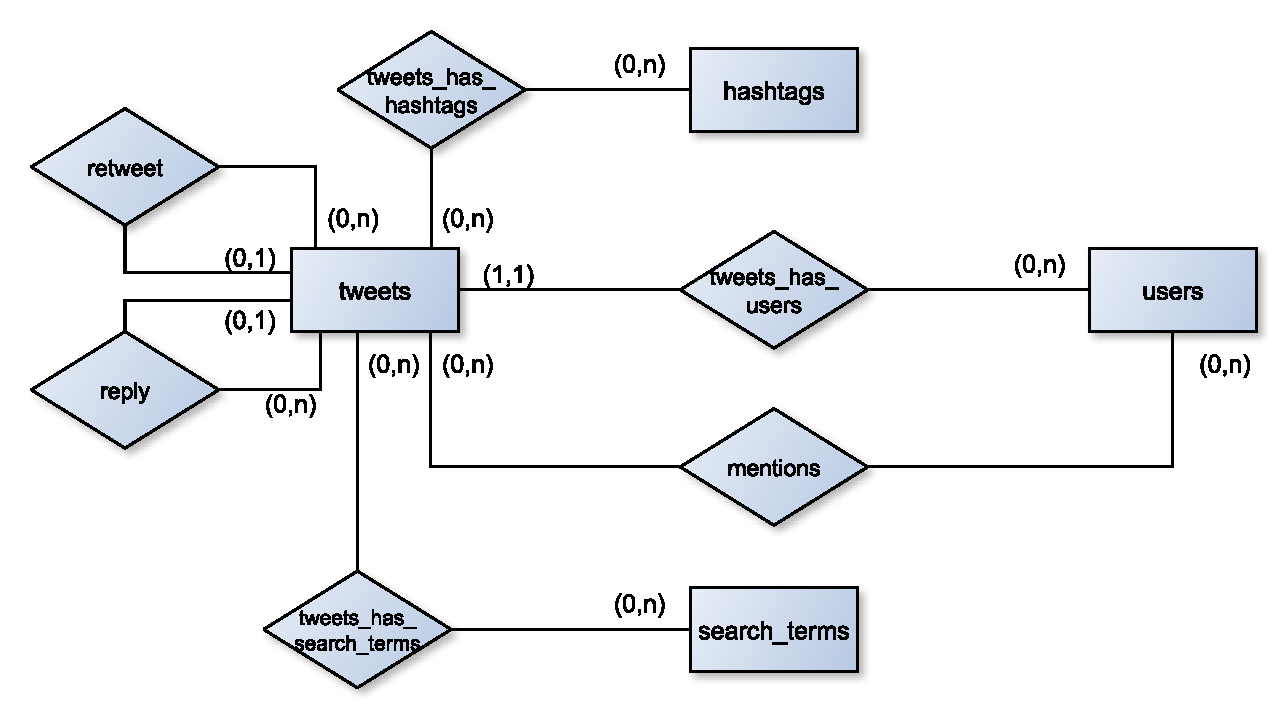
\includegraphics[width=\textwidth]{Bilder/Datenbank/ERM_Datenbank.pdf}
\caption{Bei Projektbeginn aufgestelltes Entity-Relationship-Modell}
\label{img:ERM_DB}
\end{figure}

Bei der Datenbankmodellierung wurde als erster Schritt ein Entity-Relationship-Modell aufgestellt.
Damit lassen sich die zu speichernden Twitter-Informationen zunächst auf einer konzeptionellen Ebene betrachten, die den Blick auf das Wesentliche lenkt.
Abbildung \ref{img:ERM_DB} zeigt das ER-Modell, welches zu Projektbeginn aufgestellt wurde und trotz späterer Datenbankänderungen nach wie vor die Grundstruktur zeigt.
Beispielsweise ist ein Tweet genau einem User zugeordnet, wobei ein User beliebig viele Tweets veröffentlichen kann.
Ebenso können in einem Tweet mehrere Nutzer erwähnt sein und andersherum kann ein Nutzer in mehreren Tweets erwähnt sein ($(0,n)-(0,n)$-Beziehung \texttt{mentions}).
Außerdem sind Retweets und Replies als Hierarchie modelliert, da hier eine Beziehung zwischen gleichen Entities entsteht, nämlich zwei Tweets.
Zum Beispiel bezieht sich ein Retweet immer auf einen Originaltweet, sodass einem Tweet maximal ein anderer übergeordnet werden darf.
Außerdem können einem Tweet beliebig viele Tweets untergeordnet werden (dessen Retweets).

Der einzige Entity-Typ, der sich dabei nicht direkt aus den Daten von Twitter ergibt, ist \texttt{search\_terms} mit dem Relationship-Typ \texttt{tweets\_has\_search\_terms}.
Der Entity-Typ \texttt{search\_terms} speichert die vom Nutzer eingegebenen Suchbegriffe, sowie später hinzugefügte Verwaltungsdaten für den Daemon.

Das ER-Modell wurde anschließend in ein relationales Datenbankschema überführt, welches mithilfe von MySQL Workbench erstellt wurde.
Dieses Programm erlaubt die direkte Generierung der SQL-Statements, um die entsprechende Datenbank zu erstellen. 
Den ersten Entwurf des Schemas zeigt Abbildung \ref{img:schemadb1}.

\begin{figure}[!ht]
\centering
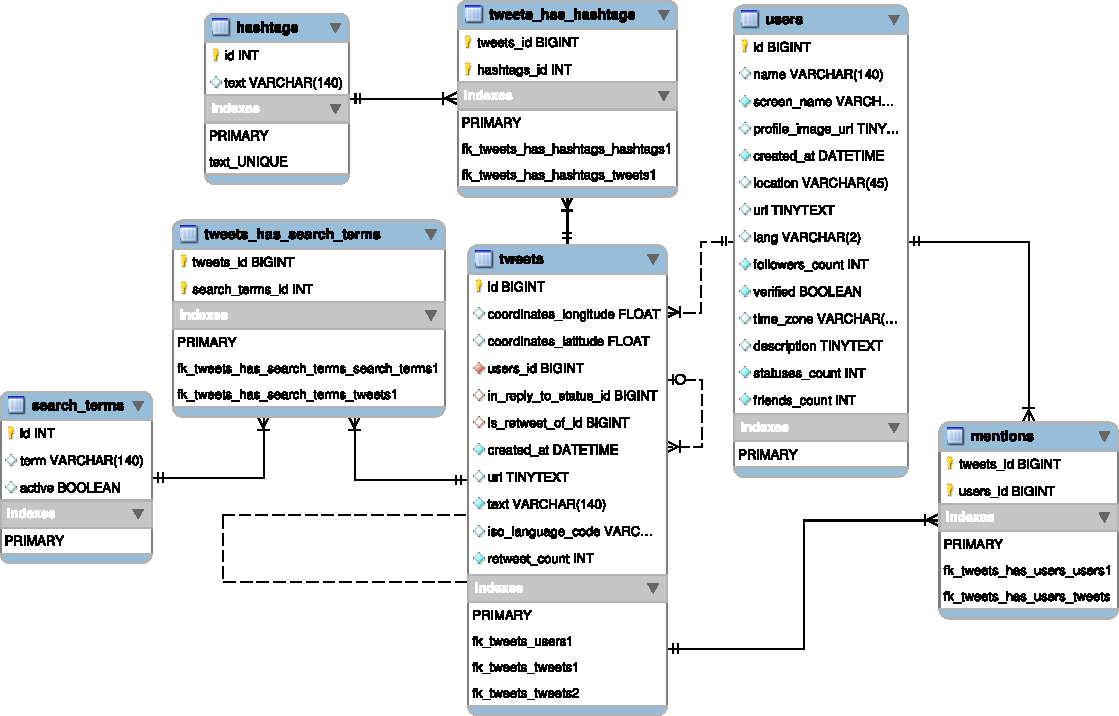
\includegraphics[width=0.9\textwidth]{Bilder/Datenbank/SchemaErsteIteration.pdf}
\caption{Erstes relationale Datenbankschema}
\label{img:schemadb1}
\end{figure}

Zum Beispiel ist zu erkennen, dass die Beziehung \texttt{tweets\_has\_users} im ER-Model nicht in einer eigenen Tabelle resultiert.
Stattdessen enthält die \texttt{tweets}-Tabelle eine zusätzliche Spalte \texttt{users\_id}, die als Fremdschlüssel auf die \texttt{users}-Tabelle referenziert.
Die beiden Hierarchien \texttt{retweet} und \texttt{reply} sind auf die gleiche Weise überführt worden.
Dagegen resultiert die \texttt{mentions}-Beziehung aufgrund der $(0,n)-(0,n)$ Kardinalitäten in einer eigenen Tabelle. 

\subsubsection{Anpassungen des Schema}
Im Verlauf der Iterationen gab es mehrere Änderungen am Schema.
So gab es zu Beginn Probleme mit der Länge einiger Felder, gerade das Feld für den Text der Tweets war zu kurz, da Twitter die Tweets als UTF-8 kodiert, MySQL aber für UTF-8 mehr als ein Zeichen benötigt.
Größere Änderungen brachte der Daemon mit sich. Dieser braucht verschiedene Verwaltungsdaten, die der \texttt{search\_terms} Tabelle hinzugefügt wurden.
Da die Menge der hinzugefügten Daten recht gering und auch die Anzahl der Einträge der Suchbegriffe insgesamt relativ gering ist, sind dadurch keine negativen Einflüsse auf die Performance zu erwarten.
%Außerdem gab es durchaus sich widersprechende Änderungen, da eine Funktionalität zuerst ausprobiert und dann wieder verworfen wurde.
In der letzten Iteration wurde noch eine Denormalisierung des Schemas aus Performance-Gründen eingeführt. 
Auf das Lösen der Performance-Probleme geht der nächste Abschnitt \ref{ssec:Performance} genauer ein.
Unser endgültiges Schema zeigt Abbildung \ref{img:schemadbfinal}.
\begin{figure}[ht]
\centering
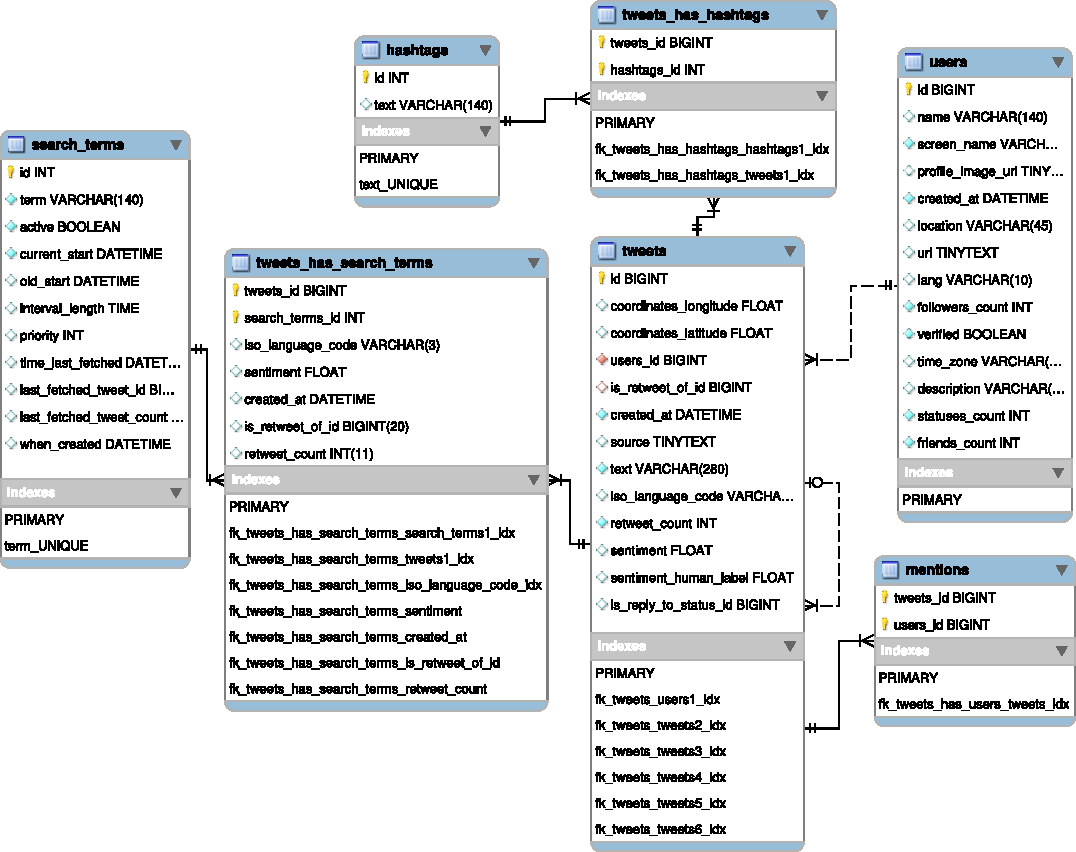
\includegraphics[width=0.8\textwidth]{Bilder/Datenbank/SchemaLetzteIteration.pdf}
\caption{Finales relationale Datenbankschema}
\label{img:schemadbfinal}
\end{figure}
Dabei ist zu sehen das die meisten Änderungen, im Vergleich zur ersten Version, an der \texttt{search\_terms}- und \texttt{tweets\_has\_search\_terms}-Tabelle stattgefunden haben.

\subsubsection{Probleme mit UTF-8}
%Gerade am Anfang gab es Probleme mit UTF-8.
Der Text von Tweets, aber auch Selbstbeschreibungen der User und andere Texte sind bei Twitter UTF-8-kodiert.
MySQL unterstützt zwar UTF-8, unterscheidet dabei aber zwei Versionen.
Die \texttt{utf8} genannte Version verwendet dabei nur 3 Byte pro Zeichen und unterstützt deswegen nicht den ganzen Umfang von UTF-8. Daher fehlen z.\,B. \textit{emoji} und weitere Zeichen, die mit 4 Byte kodiert werden.
Der bei MySQL \texttt{utf8mb4} genannte Zeichensatz verwendet hingegen 4 Byte pro Zeichen und ist deswegen in der Lage alle Zeichen von UTF-8 darzustellen.
Dieser Zeichensatz wird ab MySQL-Version 5.5 unterstützt, während frühere Versionen nur \texttt{utf8} unterstützen. Die Unterschiede werden auch in der MySQL-Dokumentation \cite{MySQLutf8} erläutert.
Da viele Tweets aus dem asiatischen Raum nicht vom \texttt{utf8}-Zeichensatz unterstütze Zeichen und viele \textit{emoji} enthalten, musste MySQL auf Version 5.5 aktualisiert werden und das Schema auf \texttt{utf8mb4} umgestellt werden.

\subsection{Performance}
\label{ssec:Performance}
Ein großes Thema für uns war die Performance der Datenbank.
Sobald der Daemon genug Tweets gesammelt hatte, stellte sich heraus, dass die Performance der Anwendung, insbesondere der Datenbank, nicht unseren Ansprüchen genügte.
Deshalb wurde das MySQL-\textit{Slow-Log} aktiviert, um langsame Abfragen zu identifizieren.
Dabei stellte sich heraus, dass ein großer Teil unserer Abfragen langsam war und nicht nur vereinzelte.
Problematisch war dabei nur die Ausführungszeit der Abfragen selbst, nicht die Zeit, in der \textit{locks} gehalten werden.

\subsubsection{Indizes}
Als erster Lösungsansatz wurde für jede Spalte separat untersucht, ob das Nutzen von Indizes sich positiv auf die Laufzeit der Abfrage, welche auf die entsprechende Spalte zugreift, auswirkt.
In einigen Fällen konnten so erhebliche Steigerungen festgestellt werden, sodass ein entsprechender Index für die Spalte angelegt wurde.
So gibt es zum Beispiel eine Abfrage, die einen Wert aus jeder Zeile aufsummiert, welche nicht vom Index profitiert.

\subsubsection{Unterabfragen}
Trotz der Indizierung einiger Spalten in der Datenbank hatten einige Abfragen noch eine sehr hohe Laufzeit. Der Grund dafür  sind die aufwändigen Joins der Tabellen. Damit weniger Datensätze in einem Join verbunden werden müssen, wurden Unterabfragen eingeführt. So wurden zum Beispiel vor dieser Veränderung zuerst alle Datensätze der \texttt{tweets}-Tabelle mit der \texttt{tweets\_has\_search\_terms} gejoint und danach erst die Einschränkungen im \texttt{where}-Teil der Abfrage ausgewertet. Eine Verwendung von Unterabfragen führt dazu, dass die Einschränkungen vor dem Join ausgewertet werden und nur die relevanten Datensätze mit der \texttt{tweets\_has\_search\_terms} verbunden werden. Dadurch wurde zum einen die Zeit verringert, die benötigt wird, um den Join durchzuführen. Ebenfalls wird der Speicherbedarf der Anfrage im RAM verringert.
Teilweise konnte dabei dennoch beobachtet werden, dass MySQL die temporären Tabellen auf die Festplatten auslagert, weil sie zu groß für das RAM waren.

%Grund war meistens, dass es sich um sehr große Tabellen handelte, weil es sehr viele Tweets zu einem Thema gab, oder noch besondere Operationen wie Sortieren auf den Daten ausgeführt werden mussten.
%In einigen Fällen war es möglich, die Abfragen selbst anzupassen um die Laufzeit zu verbessern.
%Gerade der Einsatz von Unterabfragen konnte die Laufzeit einiger Abfragen verbessern.

\subsubsection{Denormalisierung}
Um das Problem der zu großen Tabellen weiter zu lösen, wurde in der letzten Iteration beschlossen, das Schema zu denormalisieren und einige Werte, die ursprünglich ausschließlich in der \texttt{tweets}-Tabelle standen, in die \texttt{tweets\_has\_search\_terms}-Tabelle zu übernehmen. Hierdurch konnte der Join dieser beiden Tabellen in vielen Abfragen vermieden werden. Dies bewirkte eine weitere Verkleinerung der temporären Tabellen.
Die Änderungen sowohl an der Datenbank als auch an der Anwendung waren vergleichsweise klein und schnell umzusetzen und brachten an vielen Stellen bemerkbare Performanceverbesserungen.

%Ein weiteres Problem, das identifiziert werden konnte war, dass viele Queries mit hoher Laufzeit die mehrere Tabellen, insbesondere die Tweets-Tabelle, mit anderen gejoined haben.
%Da die Tweets-Tabelle die größte Tabelle ist, ist dies sehr langsam.
%Deswegen wurde unter dem Zeitdruck der letzten Iteration beschlossen, 


\subsubsection{Zählen, Sortieren und weiteres}
Aufgrund der Anforderungen der Auswertung, wie zum Beispiel vielen zeitlichen Verläufen, gibt es viele Abfragen, die Felder in den Tabellen zählen und teilweise auch sortieren müssen. Diese Funktionen von MySQL sind aber für die Anzahl an Datensätzen, die in unserer Datenbank vorliegen, ineffizient.
Um diesen Flaschenhals zu entfernen, müssten die entsprechenden Werte in einer separaten Tabelle gespeichert werden. Das Speichern dieser Werte müsste vom Daemon übernommen werden. Hierbei würde zum Beispiel die Anzahl der Tweets zu einem Suchbegriff inkrementell berechnet und abgespeichert. Da solche so genannten \textit{rollup}-Tabellen größere Veränderungen sowohl am Schema als auch am Daemon erfordert hätten, wurde aus Zeitgründen darauf verzichtet.

%In diesem Fall lassen sich die Abfragen nicht anpassen, ohne die ganze Auswertung anzupassen oder die aufsummierten Werte, z.B. in einer extra Tabelle, zwischenzuspeichern.

%Prinzipiell hätte eine Erweiterung des Schemas um eine oder mehrere Tabellen mit Metadaten, die in sehr kurzer Zeit abgefragt werden können, aber relativ großes Potential.
%Dafür hätte aber sowohl das Schema als auch die Anwendung so stark angepasst werden müssen, dass dafür die Zeit nicht reichte.

\subsubsection{Dirty Reads}
Ein weiteres Problem war, dass die Ausführungszeit der Abfragen stark abnimmt, sobald der Daemon Tweets in der Datenbank speichert.
Da die Abfragen immer erst warten, bis der Daemon die neuen Werte gespeichert hat, konnte dies die Ausführungszeit deutlich erhöhen.
Da die Abfrage selbst aber nicht auf die allerneusten Tweets angewiesen ist, zumal die Tweets, die der Daemon einspeichert ja zu ganzen anderen Suchbegriffen gehören können, wurden die sogenannten \textit{dirty reads} aktiviert.
Dabei kann eine Abfrage die Daten lesen, selbst wenn der Daemon momentan weitere Datensätze in die Tabelle schreibt. Dies kann dazu führen, dass die Abfragen nicht alle relevanten Datensätze zurückgeben.
Für den Großteil der Anfragen können wir mit diesen gegebenenfalls inkonsistenten Werten aber ohne Probleme arbeiten.
Diese Veränderung löst das Problem der Datenbankanfragen, die selbst eine lange Anfragezeit haben, allerdings nicht. Lediglich die Auswirkungen gleichzeitiger Schreibe- und Lese-Operationen können so gemindert werden.

\subsubsection{Fazit}
Die Datenbank hat im Laufe des Projektseminars mehrere Iterationen durchlaufen. 
Zum Ende des Projekts lässt sich zusammenfassen, dass die Performance weiter gesteigert werden muss, um insbesondere den Anforderungen einer Echtzeitanwendung gerecht zu werden. 
Die Veränderungen haben bereits deutliche 
Verbesserungen zur Folge gehabt.
Ein möglicher nächster Schritt wäre die weitere De- und anschließend erneute Normalisierung des Schemas, 
um zum Beispiel die oft abgefragten von den selten abgefragten Daten zu trennen, oder die Einführung 
der oben erwähnten \textit{rollup}-Tabellen für Metadaten, wie Summen von Tweets.
%Es gab einige Veränderungen, die teilweise deutliche Verbesserungen gebracht haben.
%Auch die Denormalisierung hat die Performance nochmal verbessert.
%Aber auch die Summe aller Verbesserungen war noch nicht so gut, dass man das Ganze als ein fertiges Produkt betrachten könnte.
%Das Verbessern der Performance ist also noch keineswegs abgeschlossen. 

%Entweder indem große, selten genutzte Daten, wie zum Beispiel der Text bei den Tweets, von kleinen oft benutzten Metadaten getrennt werden, in der Hoffnung das dies Hilft.
%Oder indem man, mit den jetzt konkreten Anforderungen und Abfragen, die Performance unterschiedlicher Datenbanksysteme nochmal vergleicht.